%!TEX root = ../main.tex
\chapter{Analýza problematiky}
\section{Motivácia}
\paragraph{}
Mobilné zariadenia sa stávajú čoraz väčšou súčasťou našich životov. Často sú vybavené GPS i mobilným pripojením, Bluetooth, fotoaparátom, NFC scannerom, či inými technológiami. Stali sa moderným švajčiarskym nožíkom spoločnosti, využívané na prácu, vzdelávanie i zábavu. Vďaka nim sa všetky vzdialenosti skracujú. Informácie, miesta, umenie, priatelia sú na dosah ruky. A tak sa pohyb stáva určitým bonusom k životu vo svete pixelov. Prečo však nevyužiť pixely na týchto šikovných pomôckach, aby dostali ludí do pohybu?\\
Množstvo skvelých nápadov však zostáva neuskutočnených kvôli nedostatku času, finančných prostriedkov, či znalostí programovania. Preto som sa rozhodol vytvoriť framework pre tvorbu GPS online hier. Vďaka, ktorému by si každý človek mohol stvoriť vlastný svet jednoduchšie a rýchlejšie, ako pri vývoji novej hry od začiatku. Aby sa práca na vytvorenie hry prenechala nástroju, ktorý potrebuje iba nápad.

\section{Svet hier}
V tejto sekcii si rozoberieme rôzne typy hier, ktorými sa práca inšpirovala. A teda možno nájsť mnohé črty v hrách, vytvorených pomocou tohto nástroja, práve v týchto druhoch hier. 

\subsection{MMORPG}
Massive multiplayer online role playing game - je typ hry, ktorá je založená na veľkom počte hráčov hrajúcich spolu v hernom svete. Každý hráč hrá za postavu a prechádza herným svetom. Má určité atribúty, zbrane, schopnosti, či rôzne iné objekty. Postava pomocou nich získava v tomto svete skúsenosti, peniaze či objekty, plnením rôznych úloh, či porážaním nepriateľov v boji. 
Medzi najznámejšie, ktoré si môžeme spomenúť, patria World of Warcraft, EVE online, Guild Wars. Dennodenne ich hrajú milióny hráčov, ktorí spolupracujú a súperia navzájom.

\begin{figure}[h]
  \centering
  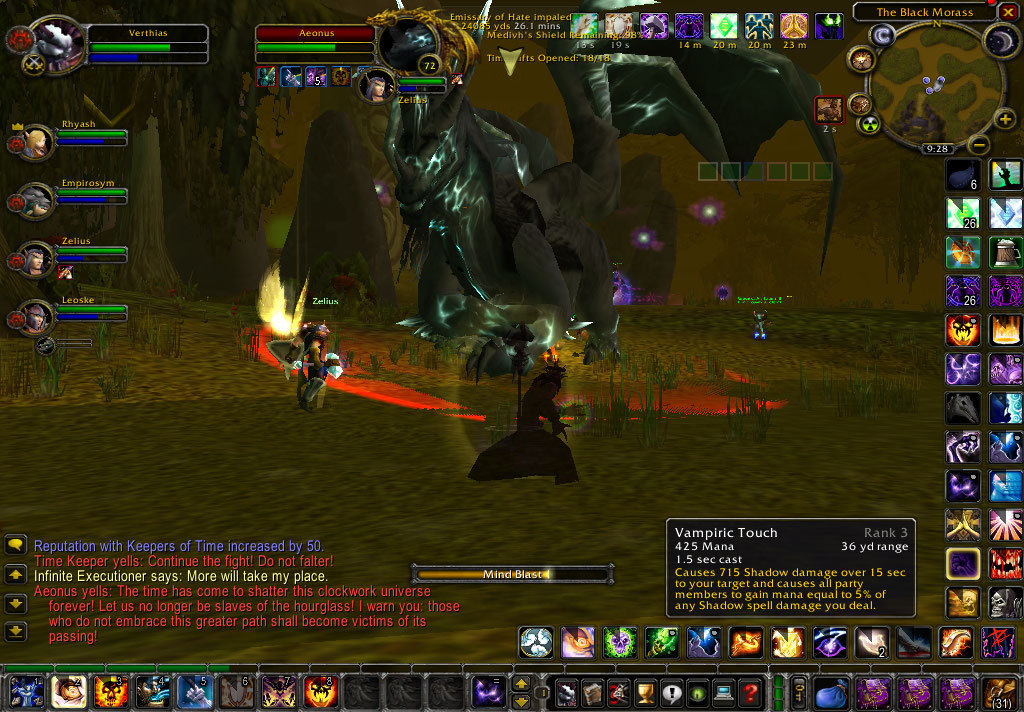
\includegraphics[height=6cm]{mainmatter/imgs/wow.jpg}
  \caption{Počítačová hra World of Warcraft}
  \label{fig:comenius}
\end{figure}


\subsection{Šifrovacie hry}
Sú súťaže, pri ktorých hráči majú za úlohu lúštiť šifry. Na stanoviskách dostanú hráči zadanie šifry, z ktorej sa po úspešnom vylúštení väčšinou dozvedia informáciu o ďaľšom stanovišti, poprípade indícii k vyriešeniu ďaľšej šifry. 

\subsection{Geocaching} 
Hra s prvkami turistiky, ktorej cieľom je nájdenie skrytého objektu (kešky) \cite{geocaching}. Jedinú informáciu, ktorú hráč má, je len poloha zadaná pomocou súradníc tohto schovaného predmetu. Často je potrebné riešiť úlohy, ktorých vyriešením hráč získa súradnice cieľa, ktorý potom môže nájsť presne pomocou GPS navigačeho zariadenia.

\section{Technológie}


\subsection{MVC} alebo model, view, controller architektúra založená na rozdelení aplikácie do týchto troch zložiek. Model je tvorený dátami, ktoré reprezentuje v aplikácii a obsahuje tiež hlavnú logiku pre prácu s nimi. View sa stará o vizuálnu stránku, ktorá je ako výsledok prezentovaná používatelovi. Controller spracováva jednotlivé dopyty od používatela a stará sa o interakciu s modelom a view. Architektúru použijeme preto, aby po implementácii herného systému, mohli tvorcovia alebo administrátori hry, zmeniť výzor aplikácie bez nebezpečenstva porušenia jej funkcionality.
\begin{figure}[h]
  \centering
  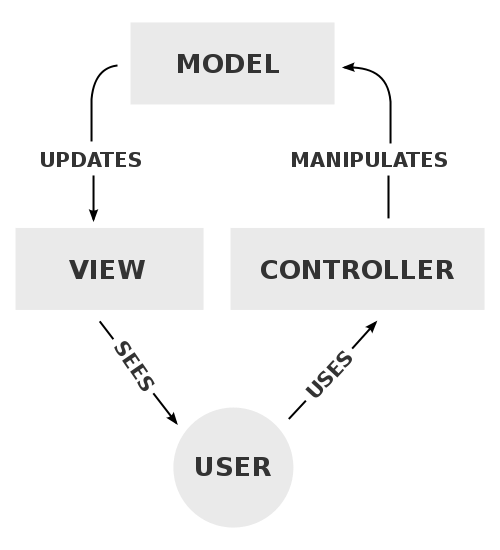
\includegraphics[height=6cm]{mainmatter/imgs/mvc.png}
  \caption{MVC architektúra}
  \label{fig:comenius}
\end{figure}

% \subsection{Android} Na strane klienta je zvolený operačný systém Android od firmy Google. Ktorý sa vačšinou používa práve na mobilných zariadeniach. Oproti konkurenčnému systému iOS od Apple je operačný systém open source. Ďalším argumentom bola politika schvalovania aplikácii a možnosť ich vyvýjať na rôznych operačných systémoch, kde pre android je to možné takmer pod každým operačným systémom. Ďaľšou možnosťou bol Windows Phone, ten však bol zavrhnutý kvôli jeho nižšiemu rozšíreniu \
% Android ma jadro založené na linuxe. Aplikácie možno vývíjať v jazyku Java pomocou Android SDK, ktorý ponúka funkcie na ovládanie zariadenia.


\subsection{Bluetooth} Radiový štandard IEEE 802.15.1, ktorý slúži tiež na bezdotykovú komunikáciu medzi zariadeniami. Bol vytvorený firmou Ericsson v roku 1994. Pomenovaný je podľa dánskeho kráľa s menom Harald Blatand (do angličtiny prelozené ako Bluetooth), ktorému sa podarilo vďaka jeho diplomatickým schopnostiam uzmieriť kmene, ktoré proti sebe bojovali. Podla typu bluetooth vysielačov/prijímačov môžu mať navzajom dosah až po 400 metrov. Najčastejšie sú však zariadenia s dosahom 10metrov. S novšími verziami bluetooth je možná rýchlosť prenosu dát až 24 Mbit za sekundu. Často sa používa na jednoduché posielanie dát medzi mobilnými zariadeniami. Pre riešenie problému komunikácie medzi hráčmi, nie je podstatná rýchlosť ani maximálna vzdialenosť technológie. Práve pre to, aby odovzávanie pôsobilo realistickejšie, je dobré aby hráči boli bližšie k sebe. Vysoke prenosové rýchlosti nie sú potrebné na odoslanie objektu s požiadavkou, medzi zariadeniami. Podstatná je práve rozšírenosť tejto technológie v mobilných zariadeniach, aby mohli všetci hráči medzi sebou komunikovať.


\subsection{QR Kódy} QR (Quick Response) sú čiarové kódy, v ktorých je uložená informácia. Boli vyvinuté japonskou automobilkou Toyota na rýchle čítanie informácii o tovare nimi označenými. Sú zložené z bielych a čiernych štvorcov, usporiadaných v mriežke. Môžu byť vytlačené na papier a prečítané pomocou čítačiek či zariadení, ktoré zosnímajú kód a dokážu ho preložiť späť do pôvodnej informácie.  QR kódy sú často pridávané do reklamných plagátov, či videí ako odkazy na produkty výrobcu. Nájdeme ich ale i pri kultúrnych pamiatkach ako ďaľší zdroj informacií. Využitia sú rôzne, kedže na relatívne malej ploche dokážu uložit 7089 numerických, 4296 alfanumerických, 2953 binárnych, či 1817 kanji znakov\cite{qrcode-about}. QR kódy obsahujú tiež opravu chýb pri mierne poškodenom QR kóde a tak je čítačka schopná prečítať informáciu aj keď je kúsok QR kódu prekrytý až do 30\% plochy \cite{qrcode-about}. Pomocou pridaného loga ku QR kódu hry bude táto vlastnosť QR kódov využívaná pre ich lepšiu identifikáciu.

\subsection{NFC} Mnoho ľudí možno ani netuší, že sa už s NFC stretli. Napríklad ak platili pri nákupoch pomocou karty bezdotykovo. NFC (Near field communcation) je pomerne mladá technológia, pomocou ktorej môžu zariadenia medzi sebou komunikovať na krátku vzdialenosť (maximálne 20 centimetrov), bezdotykovo. Je potomkom RFID - Rádiofrekvenčných identifikačných kariet a ich čítačiek, ktoré sa spojili v NFC v smartfónoch. Takže zariadenia vybavené touto technológiou sú schopné zapisovať a čítať NFC tagy a komunikovať s ostatnými zariadeniami, ktoré NFC majú. Výhodou použitia tejto technológie by bola jednoduchosť použitia. Nevýhodou je pomerne malé množstvo starších zariadení, ktoré podporujú túto technológiu.

\section{Frameworky, knižnice a API}
V tejto práci bolo podstatné využiť knižnice, ktoré urýchlia jej vývoj a ich používanie nebude spoplatnené.

\subsection{Codeigniter} Open sourceovy(OSL) PHP framework. Zakladá si na MVC architektúre, avšak necháva volnosť programátorovi. Taktiež ako ďaľšiu z klúčových vlastností pre jeho výber bola jeho rýchlosť\cite{codeigniter-guide}. Bol založený v roku 2006 a je vyvíjaný americkou firmou EllisLab. Jej ďaľším dôležitým prvkom sú tiež knižnice a nástroje, ktoré ulahčujú vývoj aplikacie. Jeho funkcionalitu je možné rozširovať pomocou helperov a rožširovaní tried.

\subsection{jQuery} Veľmi obľúbená\cite{jquery-usage} javascriptová knižnica, ktorá uľahčuje prácu hlavne pri manipulovaní s objektami na stránke. Často sa teda využíva pri tvorbe efektov, či žjednodušovaní vývoja aplikácií, využívajúcich javascript. jQuery sa o to všetko snaží pri zachovávaní kompatibility medzi rôznymi internetovými prehliadačmi\cite{jquery-browsers}. Podporuje množstvo rozšírení pomocou pluginov\cite{jquery-plugins}. jQuery je opensource projekt, vydavaný pod MIT licenciou. 

\subsection{Bootstrap} Front-endový framework pre tvorbu webových stránok. Je vytvorený pomocou HTML a CSS. Bol založený členmi vývojového tímu Twitteru a v roku 2011 vydaný ako opensource projekt\cite{bootstrap-about}. Obsahuje rôzne šablóny pre dizajn rôznych komponentov na webových stránkach ako sú napríklad gombíky, formy, navigácie. Bootstrap podporuje responzívny design. Responzívne stránky sa teda môžu prispôsobovať pre jednotlivé zariadenia s rôznymi rozlíšeniami obrazoviek. Poslúži nám na vytvorenie moderného a funkčného designu, ktorý bude podporovaný medzi rôznymi webovými prehliadačmi.


\subsection{Google maps} Služba od internetového giganta Google, pomocou ktorej sa dá zobraziť mapa réalneho sveta ale i regióny toho fiktívneho - herného. Mapy sú poskytované pomocou Javscriptu, CSS a HTML. Táto API má však svoje obmedzenie pri používaní zadarmo - 25 000 načítaní za deň\cite{gmaps-usage}. Toto obmedzenie nie je kritické, pretože tvorcovia hry môžu nastaviť kľúč pomocou, ktorého je identifikovaný používateľ tejto služby. To znamená, že ak by tvorcov limit obmedzoval, môžu si ho navýšiť zmenou plánu, ktorý v tejto službe používajú. 

\subsection{QR code generator} Na strane serveru je knižnica jasnou voľbou pre jej množstvo funkcií a parametrov \cite{qrgenerator-functions}, ktoré poskytuje pri tvorbe QR kódov. Knižnica bude musieť byť upravená pre použitie vo frameworku \emph{CodeIgniter}. QR kódy budú môcť byť automaticky generované systémom a tvorcovia hry ich budú môcť vytlačiť a pridať ich do herného prostredia, kde sa hra bude odohrávať. Napríklad budú môcť vytvoriť úlohu, či odmenu, ktorá sa predá hráčovi, ktorý ju naskenoval.



\subsection{ZBar} GPL knižnica pre Android, pomocou ktorej je možné skenovať a rozoznávať QR kódy. Táto knižnica bola vybraná, napriek obľúbenej knižnici \emph{ZXing}. Tá totiž pre svoje použitie potrebuje stiahnúť aplikáciu, ktorej sa posiela požiadavok. Preto aby sme sa vyhli potrebe inštalácie ďaľšej aplikácie, je najvhodnejšie riešenie pomocou tejto knižnice. \emph{ZBar} je tiež relatívne jednoduché zakomponovať do aplikácie. \cite{qrreader}.

\subsection{Iconify}
Knižnica, ktorá slúži na jednoduché používanie fontu Font Awesome v android aplikácii. Pomocou tejto knižnice môžeme spraviť omnoho intuitívnejšie ovládanie aplikácie pre používateľa, vďaka obrázkom, priradením k textu na akčných tlačidlách.


\section{Prehľad existujúcich aplikácií}
V tejto sekcií sa pozrieme na existujúce aplikácie, ktoré sa zaoberajú podobnou problematikou ako táto práca. Keďže aplikácia alebo framework, ktoré by riešili tvorbu GPS online hier pre android neexistujú, budú analyzované existujúce nástroje na tvorbu hier a potom hry samotné pričom budú spomenuté ich silné a slabé stránky vzhľadom na ciele tejto práce. 

\subsection{Nástroje na tvorbu hier}

\subsubsection{Rpg Creator} je komerčný program, ktorý používateľom umožňuje vytvárať ich vlastné dvojrozmerné RPG a MMORPG. Webová aplikácia ponúka nástroje na tvorbu hry, takže nie je potrebná žiadna inštalácia na strane tvorcu hry. Používateľ môže pridať vlastné obrázky do hry a nastaviť ovládanie postavičiek, či správanie sveta. Výsledná hra môže byť vyexportovaná na rôzne platformy(Windows, Linux, Mac OS) \cite{rpgcreator}.

\begin{figure}
  \centering
  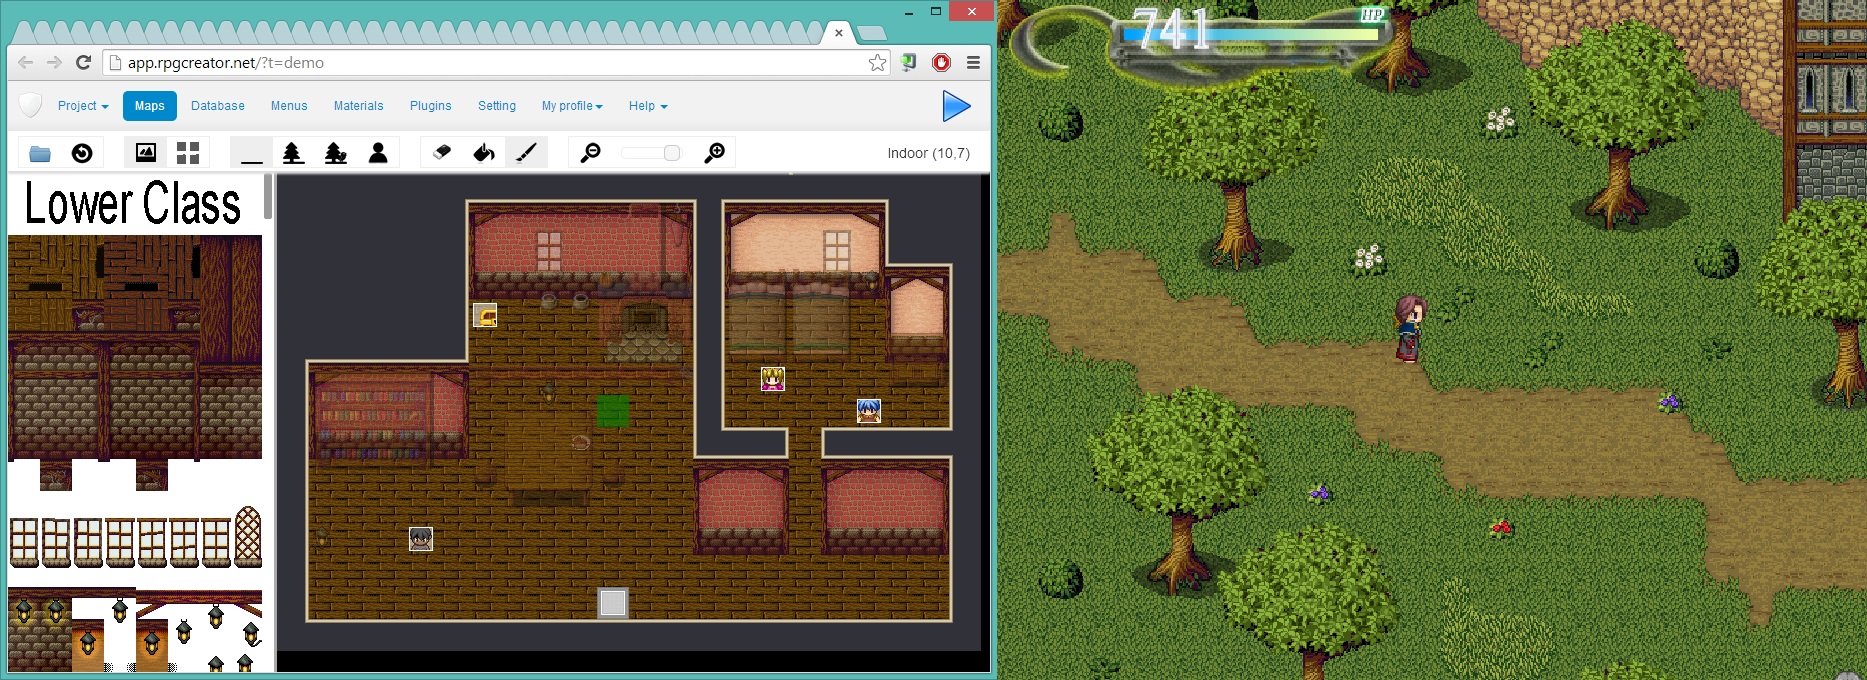
\includegraphics[width=14cm]{mainmatter/imgs/rpgcreator.png}
  \caption{Webová aplikácia po vytvorení hry ponúka možnosť spustiť hru v prehliadači}
  \label{fig:rpgcreator}
\end{figure}


\paragraph*{Silné stránky}
\begin{itemize}
  \item Webová aplikácia pre tvorbu hry
  \item Jednoduchosť používania
\end{itemize}
\paragraph*{Slabé stránky}
\begin{itemize}
  \item Platená aplikácia
  \item Chýbajúci export natívnej aplikácie pre mobilné zariadenia
\end{itemize}





\subsubsection{Rpg Maker} Komerčný program, ktorý používateľom umožňuje vytvárať ich vlastné dvojrozmerné RPG na počítač. Napriek tomu, že herný engine je určený hlavne na tvorbu hier tohto žánru sa v ňom dajú vytvárať aj hry žánrov iných - napríklad adventúry \cite{rpg-maker-game}. Obsahuje editor s predrobeným balíkom textúr a obrázkov postavičiek. Používatel však môže pridať i vlastné. 
\cite{rpg-maker}
\begin{figure}
  \centering
  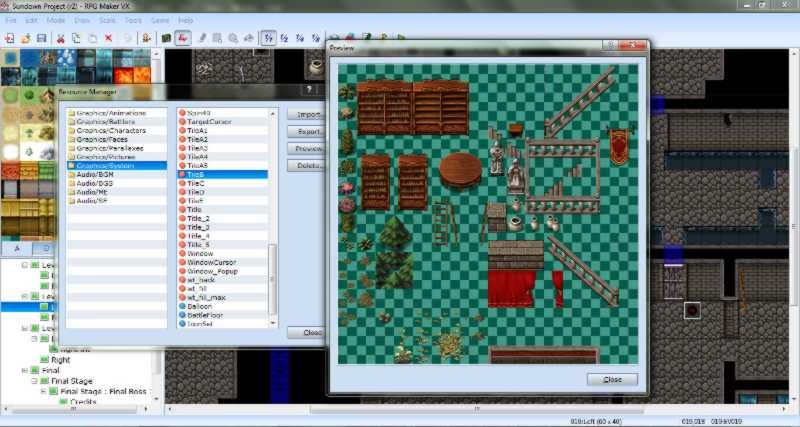
\includegraphics[width=14cm]{mainmatter/imgs/rpgmaker.jpg}
  \caption{Platený nástroj RPG Maker ponuká jednoduché prostredie na tvorbu 2D RPG hier}
  \label{fig:comenius}
\end{figure}


\subsection{Hry}


\subsubsection{Ingress} Je hra pre android zariadenia z dielne Google, ktorú hrá množstvo ľudí naraz. Hra využíva princíp geocachingu, kde hráči pátrajú po ukrytých predmetoch. Hráčov pohyb je premietaný do herného sveta pomocou GPS a internetového pripojenia. Dej hry je postavený na pátraní po tajomnej energii, ktorá dokáže ovládať ľudskú myseľ. V hre existujú dve hlavné frakcie - Osvietení, vítajúci príchod energie a Odpor, ktorý sa ich snaží zastaviť. Hráči sa ako jednotlivci alebo v skupinkách snažia body s touto energiou obsadzovať. Následne získanú energiu môžu použiť na technologický pokrok, ktorý možno využiť v boji proti nepriateľskej frakcii. 

\paragraph*{Silné stránky}
\begin{itemize}
  \item Využívanie GPS
  \item Hra inšpiruje hráčov k pohybu
\end{itemize}
\paragraph*{Slabé stránky}
\begin{itemize}
  \item Slabší dej a atmosféra

\end{itemize}

\begin{figure}
  \centering
  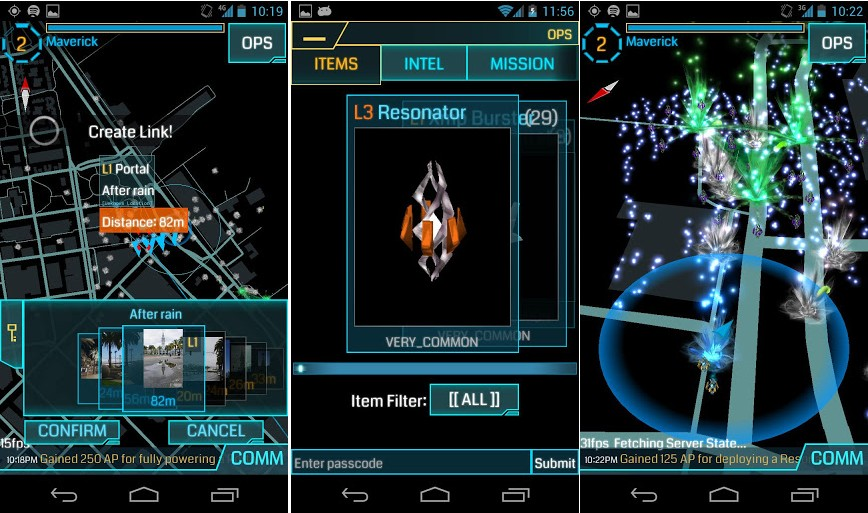
\includegraphics[height=6cm]{mainmatter/imgs/ingress.jpg}
  \caption{V hre Ingress hráči bojujú o územia}
  \label{fig:ingress}
\end{figure}



\subsubsection{Map attack!} je GPS online hra, pre mobilné zariadenia Android a iPhone \cite{mapattack}. Herná plocha sa nachádza vonku. Na tejto ploche dva tímy súperia o zabratie najväčšieho počtu menších plôch - bodov. Tím, ktorý ma viac bodov za určitý čas, vyhráva. Hra neuvádza hráčov do herného príbehu a nedáva hráčom možnosť riešiť konkrétne úlohy. Nie je to však zápor, jedná sa o črtu hry, ktorá pripominá skupinovú naháňačku, a preto nie sú potrebné tieto vlastnosti.
\begin{figure}[h]
  \centering
  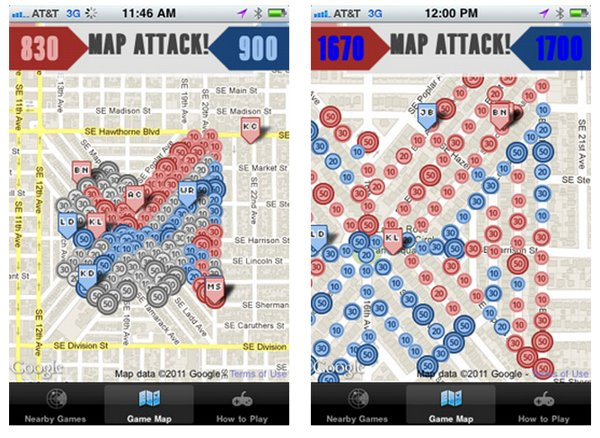
\includegraphics[height=6cm]{mainmatter/imgs/mapatack.jpg}
  \caption{Dva tímy, obsadzujúce územia v hre Map attack! }
  \label{fig:mapatack}
\end{figure}

\paragraph*{Silné stránky}
\begin{itemize}
  \item Pre Android i iOS
  \item Zadarmo   
  \item Využívanie GPS
\end{itemize}
\paragraph*{Slabé stránky}
\begin{itemize}
  \item Zatiaľ stále nie je možné vytvoriť si vlastnú hraciu plochu  
\end{itemize}



\subsubsection{World of Warcraft} je hlavne MMORPG hra pre počítače, ktorá získala milióny hráčov, hlavne pre svoju atmosféru a hrateľnosť. Bola vytvorená firmou Blizzard \cite{wow-blizard}. Hra má klasické črty MMORPG a dáva hráčovi voľnosť, aby so svojou postavou mohol pohybovať po trojrozmernom hernom svete, kde nemusí sledovať hlavnú dejovú líniu. Navyše hráčovi ponúka mnohé možnosti interakcie s prostredím \cite{wow-blizard-guide}.
\begin{figure}[h]
  \centering
  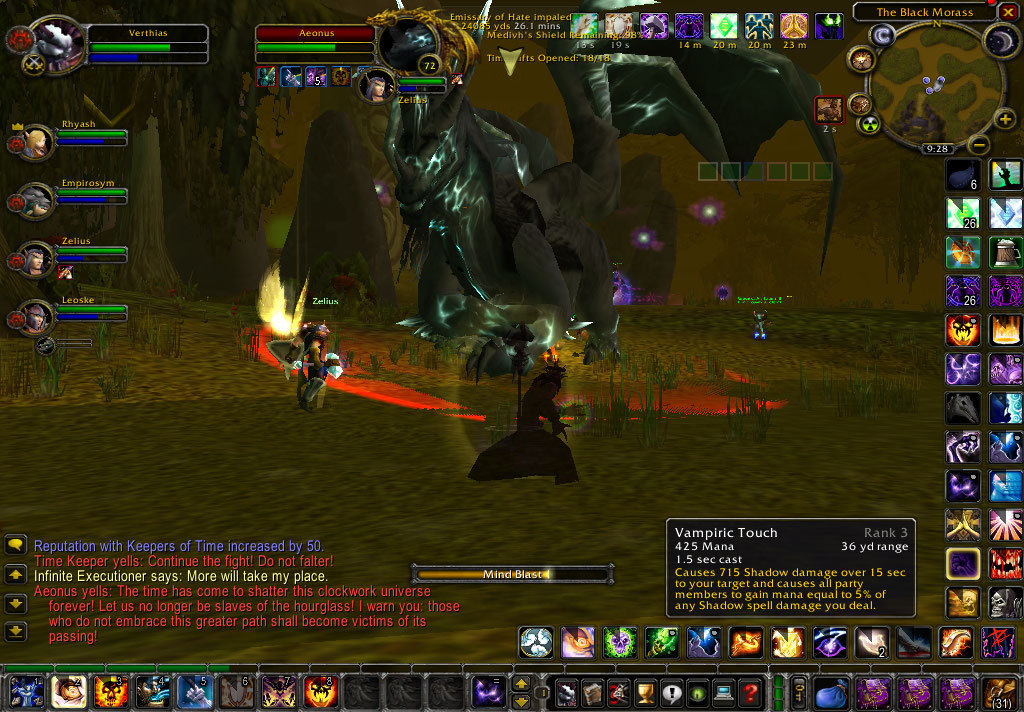
\includegraphics[height=6cm]{mainmatter/imgs/wow.jpg}
  \caption{Počítačová hra World of Warcraft}
  \label{fig:wowko}
\end{figure}

\paragraph*{Silné stránky}
\begin{itemize}
  \item Atmosféra a dej
  \item Grafika 
  \item Hrateľnosť 
\end{itemize}
\paragraph*{Slabé stránky}
\begin{itemize}
  \item Cena   
\end{itemize}